A montagem do tambor, com os esforços atuantes está ilustrada abaixo:

\begin{figure}[H]
  \centering
  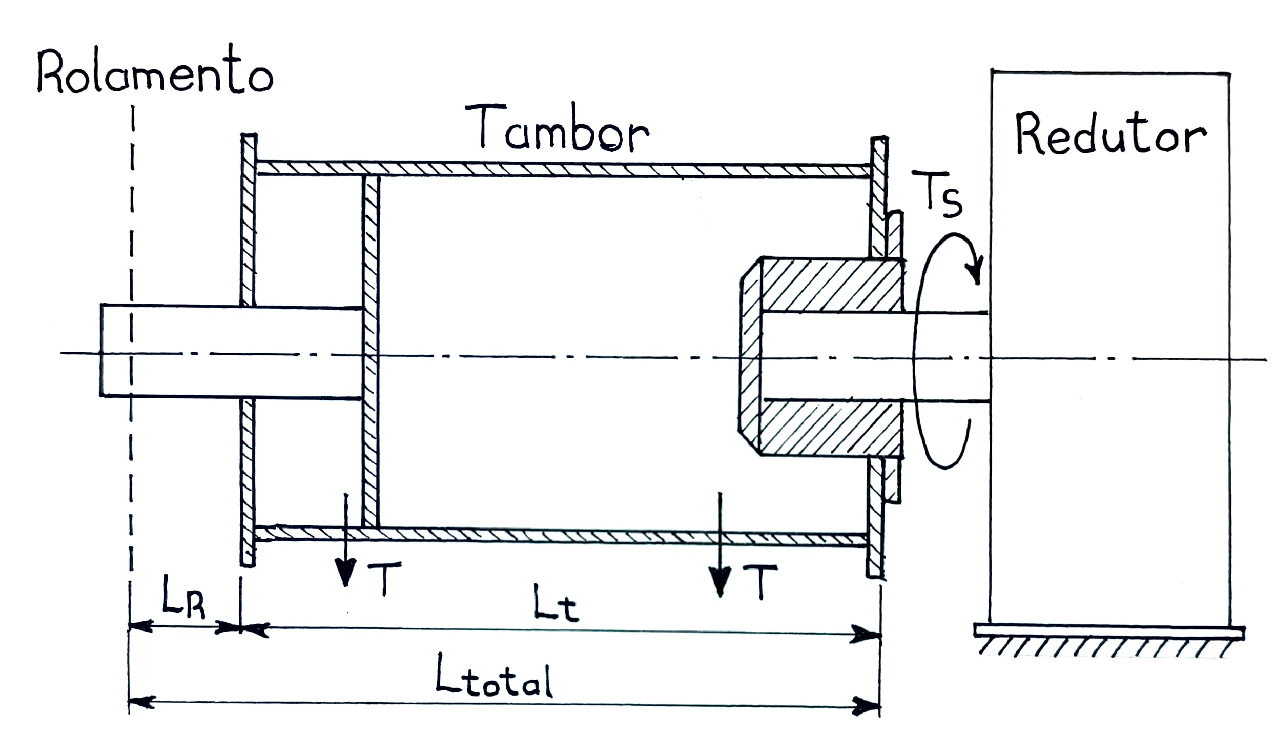
\includegraphics[width=0.8\textwidth]{content/sections/03_sistema_de_elevacao/sections/16_projeto_do_tambor/sections/01_modelagem_estatica_do_tambor/drawings/tambor_redutor.pdf}
  \caption{Representação da montagem do tambor com o redutor (Autor)}
  \label{fig:montagem_tambor}
\end{figure}

A estrutura do tambor pode ser modelada como uma viga bi apoiada, com o peso do tambor e do cabo de aço atuando em forma de carga distribuída, conforme ilustrado abaixo:

\begin{figure}[H]
  \centering
  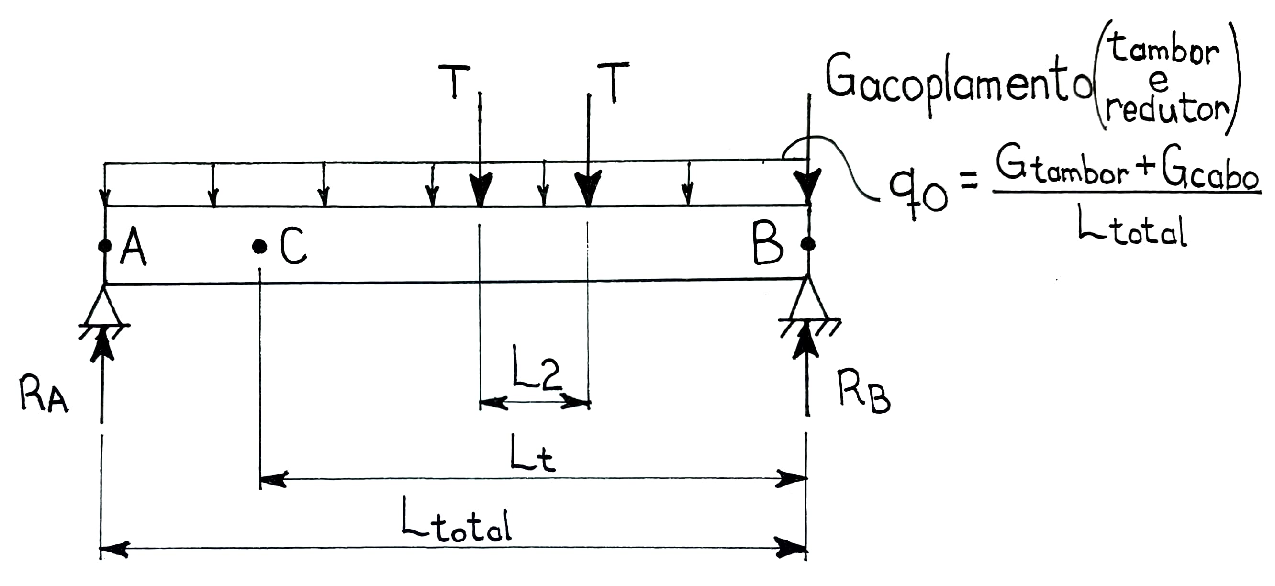
\includegraphics[width=0.8\textwidth]{content/sections/03_sistema_de_elevacao/sections/16_projeto_do_tambor/sections/01_modelagem_estatica_do_tambor/drawings/modelagem_tambor.pdf}
  \caption{Modelagem estática do tambor (Autor)}
  \label{fig:modelagem_tambor}
\end{figure}

\subsubsection{Cargas}

A tração no cabo de aço, conforme calculada na Seção \ref{sec:forca_de_tracao_no_cabo}, é de \SI{25377,8}{\newton}.

O peso do acoplamento redutor-tambor, obtido no catálogo (Tabela \ref{tab:dados_acoplamento_tambor}), é de \SI{54}{\kilogram}, equivalente a \SI{540}{\newton}.

O peso do tambor, conforme calculado na Seção \ref{sec:peso_do_tambor}, é de \SI{6611,851}{\newton}.

Já o peso do cabo de aço, conforme calculado na Seção \ref{sec:peso_do_cabo_de_aco}, é de \SI{978,48}{\newton}.

A carga distribuída considerada na modelagem estática é dada por:

\begin{equation}
  q_o = \frac{G_{\text{tambor}} + G_{\text{cabo}}}{L_{\text{total}}}
  \label{eq:carga_distribuida_tambor}
\end{equation}

\begin{align*}
  q_o & = \frac{6611,85 + 978,48}{2,212} \\
  q_o & = \boxed{\SI{3431,4}{\newton/m}}
\end{align*}

As cargas atuantes consideradas no dimensionamento do tambor estão resumidas abaixo:

\begin{table}[H]
  \centering
  \caption{Cargas atuantes no tambor}
  \label{tab:cargas_atuantes_tambor}
  \begin{tabularx}{\textwidth}{>{\centering\arraybackslash}X>{\centering\arraybackslash}X>{\centering\arraybackslash}X}
    \toprule
    Descrição                          & Símbolo                  & Valor                  \\
    \midrule
    Tração no cabo de aço              & $T$                      & \SI{25377,8}{\newton}  \\
    Peso do acoplamento redutor-tambor & $G_{\text{acoplamento}}$ & \SI{540}{\newton}      \\
    Peso do tambor                     & $G_{\text{tambor}}$      & \SI{6611,85}{\newton}  \\
    Peso do cabo de aço                & $G_{\text{cabo}}$        & \SI{978,48}{\newton}   \\
    Carga distribuída                  & $q_o$                    & \SI{3431,4}{\newton/m} \\
    \bottomrule
  \end{tabularx}
\end{table}

\subsubsection{Distâncias}

As distâncias consideradas na modelagem estática são:

\begin{table}[H]
  \centering
  \caption{Distâncias consideradas na modelagem estática}
  \label{tab:distancias_consideradas_modelagem_estatica}
  \begin{tabularx}{\textwidth}{>{\centering\arraybackslash}X>{\centering\arraybackslash}X>{\centering\arraybackslash}X}
    \toprule
    Descrição                             & Símbolo            & Valor              \\
    \midrule
    Espaçamento central entre as ranhuras & $L_2$              & \SI{0,2}{\meter}   \\
    Comprimento do tambor                 & $L_t$              & \SI{2,112}{\meter} \\
    Comprimento total                     & $L_{\text{total}}$ & \SI{2,212}{\meter} \\
    \bottomrule
  \end{tabularx}
\end{table}

\subsubsection{Diagrama de Corpo Livre}

Com base nas cargas e distâncias consideradas, o diagrama de corpo livre do tambor é ilustrado abaixo:

\begin{figure}[H]
  \centering
  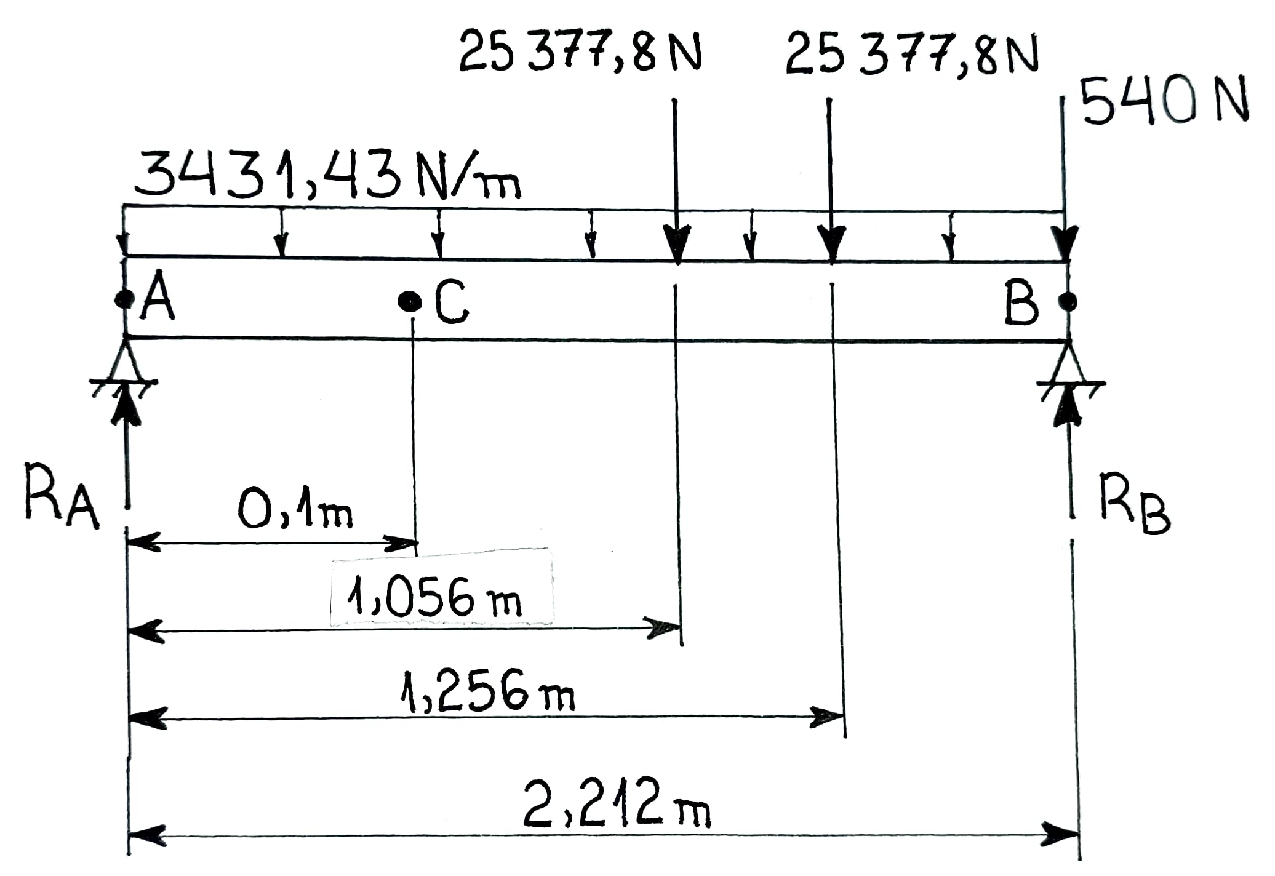
\includegraphics[width=0.8\textwidth]{content/sections/03_sistema_de_elevacao/sections/16_projeto_do_tambor/sections/01_modelagem_estatica_do_tambor/drawings/dcl_tambor.pdf}
  \caption{DCL do tambor (Autor)}
  \label{fig:dcl_tambor}
\end{figure}

\subsubsection{Reações de Apoio}

Utilizando as equações de equilíbrio, as reações de apoio podem ser calculadas.

Os momentos atuantes no ponto A são:

\begin{equation*}
  2,212 \cdot R_B
\end{equation*}

\begin{equation*}
  - 3431,43 \cdot \frac{2,212}{2} \cdot 2,212 = \SI{-8394,9}{\newton\meter}
\end{equation*}

\begin{equation*}
  - 1,056 \cdot 25377,8 = \SI{-26798,96}{\newton\meter}
\end{equation*}

\begin{equation*}
  - 1,256 \cdot 25377,8 = \SI{-31874,52}{\newton\meter}
\end{equation*}

\begin{equation*}
  - 2,212 \cdot 540 = \SI{-1194,48}{\newton\meter}
\end{equation*}

\vspace{1em}

Aplicando nas equações de equilíbrio, temos:

\begin{flalign*}
   & \sum M_A = 0                                           &  & \\
   & 2,212 R_B - 8394,9 - 26798,96 - 31874,52 - 1194,48 = 0 &  &
\end{flalign*}

\begin{equation}
  2,212 R_B - 68262,86 = 0
  \label{eq:sum_ma_tambor}
\end{equation}

\vspace{1em}

\begin{flalign*}
   & \sum F_y = 0                                                &  & \\
   & R_A + R_B - 3431,43 \cdot 2,212 - 2 \cdot 25377,8 - 540 = 0 &  &
\end{flalign*}

\begin{equation}
  R_A + R_B - 58885,92 = 0
  \label{eq:sum_fy_tambor}
\end{equation}

\vspace{1em}

Desenvolvendo a equação \eqref{eq:sum_ma_tambor}, temos:

\begin{align*}
  R_B & = \frac{68262,86}{2,212}         \\
  R_B & = \boxed{\SI{30860,24}{\newton}}
\end{align*}

\vspace{1em}

Substituindo o valor de $R_B$ na equação \eqref{eq:sum_fy_tambor}, temos:

\begin{align*}
  R_A & = 58885,92 - 30860,24            \\
  R_A & = \boxed{\SI{28025,68}{\newton}}
\end{align*}

\vspace{1em}

\subsubsection{Funções de Singularidade}

Para obter as equações dos esforços internos de força cortante e momento fletor, utilizou-se o método das funções de singularidade de Macaulay.

\begin{align*}
  V(x) & = -3431,43 \left<x\right>^1              \\
       & \quad + 28025,68 \left<x\right>^0        \\
       & \quad - 25377,8 \left<x - 1,056\right>^0
\end{align*}
